\documentclass[article,paper=a4paper]{jlreq}

% jpreportパッケージの読み込み
\usepackage{jpreport}

% ページレイアウトの設定
\usepackage{geometry}
\usepackage{enumitem}
\geometry{
    top=25mm,
    bottom=25mm,
    left=25mm,
    right=25mm
}
% TikZライブラリ
\usetikzlibrary{
    patterns,
    calc,
    arrows,
    decorations,
    angles,
    shapes.geometric,
    fit,
    knots
}
% TikZ用のスタイル
\tikzset{
  every path/.style={
    black,
    line width=2pt
  },
  every node/.style={
    transform shape,
    knot crossing,
    inner sep=1.5pt
  }
}
% ハイパーリンクの設定
\usepackage[unicode]{hyperref}
\usepackage{bookmark}
\usepackage[nameinlink]{cleveref}

\hypersetup{
    colorlinks=true,
    linkcolor=black,
    urlcolor=blue,
    citecolor=blue,
    pdftitle=,
    pdfauthor=
}

% 数学演算子の定義


% cleveref用の日本語設定
\crefname{thm}{定理}{定理}
\crefname{lem}{補題}{補題}
\crefname{cor}{系}{系}
\crefname{ex}{例}{例}
\crefname{dfn}{定義}{定義}
\crefname{prop}{命題}{命題}
\crefname{prob}{問題}{問題}

% 色彩の定義
\definecolor{yukari}{RGB}{196, 163, 191}

% 文書情報
\title{微分方程式特論}
\author{akari0koutya}
\date{\today}

\begin{document}

% --- タイトル ------------------------------------------------------
\maketitle
\tableofcontents
%% 本文の内容をここに記述
% ====================================================================

\section{1回：周期関数、三角級数(2026/04/15)}
\begin{dfn}
\quad $f(x)$ : $\R$ 上の連続関数\par
すべての $x \in \R$ に対して $f(x+p) = f(x)$ となるような正の数 $p$ が存在するとき、$f$ は \textbf{周期的} であるという。このとき、$p$ を $f$ の \textbf{周期} という。
\end{dfn}

長さ $p$ におけるグラフを周期的に繰り返すことで、周期関数のグラフを得られる。

\begin{figure}[htbp]
\centering
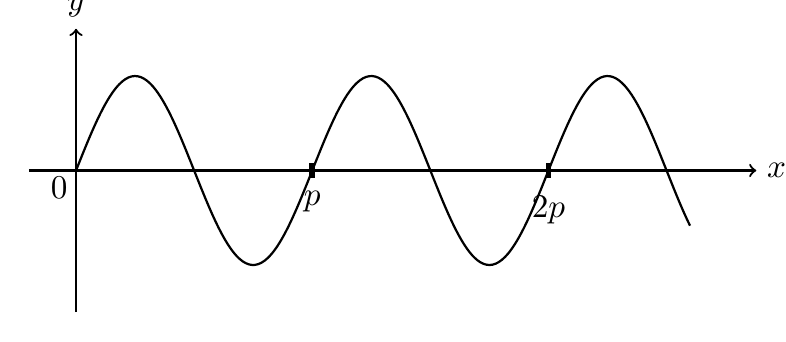
\begin{tikzpicture}[scale=1.2]
    % 周期 p の値
    \def\p{2.5}

    % 座標軸
    \draw[thick,->] (-0.5,0) -- (7.2,0) node[right] {$x$};
    \draw[thick,->] (0,-1.5) -- (0,1.5) node[above] {$y$};

    % x軸上の目盛
    \draw (\p,0.08) -- (\p,-0.08) node[below] {$p$};
    \draw ({2*\p},0.08) -- ({2*\p},-0.08) node[below] {$2p$};

    % 周期関数 y = sin(2πx/p)
    \draw[thick,domain=0:6.5,samples=200,smooth]
        plot (\x,{sin(360/\p*\x)});

    % 原点ラベル
    \node[below left] at (0,0) {$0$};
\end{tikzpicture}\caption{長さ $p$ の周期関数の例}
\end{figure}

\begin{ex}
定数関数 $f(x) = c$ は任意の正数を周期とするため、周期的。
\end{ex}

\begin{ex}
    正弦関数 $f(x) = \sin x$ および余弦関数 $f(x) = \cos x$ は周期 $2\pi$ を持つため、周期的。
\end{ex}

\begin{ex}[周期関数でない関数の例]
    $f(x) = x$ や $f(x) = e^x$ や $f(x) = \log x$は周期関数ではない。
\end{ex}

\begin{prop}
    \quad $f(x)$ : $\R$ 上の周期関数\par
    任意の整数 $n$ に対して $f(x+np) = f(x)$ が成り立つ。
\end{prop}

\begin{proof}
    $f(x+p) = f(x)$ より、$f(x+2p) = f((x+p)+p) = f(x+p) = f(x)$ となる。これを繰り返すことで、任意の正の整数 $n$ に対して $f(x+np) = f(x)$ が成り立つ。

    また、$f(x) = f((x-p)+p) = f(x-p)$ より、任意の負の整数 $n$ に対しても $f(x+np) = f(x)$ が成り立つ。
\end{proof}

このことから、周期 $p$ の関数は、 $2p$, $3p$, ... などの正の整数倍の周期も持つことがわかる。

\begin{prop}
    \quad $f(x)$, $g(x)$ : $\R$ 上の周期関数\par
    このとき、任意の定数 $\alpha$, $\beta$ に対して、$h(x) = \alpha f(x) + \beta g(x)$ も周期関数である。
\end{prop}

\begin{proof}
    \[h(x+p) = \alpha f(x+p) + \beta g(x+p) = \alpha f(x) + \beta g(x) = h(x)\]
    より、$h$ は周期関数である。
\end{proof}

\begin{dfn}
    周期関数 $f$ の周期のうち、最小のものを $f$ の \textbf{基本周期} という。
\end{dfn}

\begin{thm}
    \quad $f(x)$ : $\R$ 上の"いい"周期関数\par
    このとき、
    \[f(x) = \frac{a_0}{2} + \sum_{n=1}^{\infty} (a_n \cos(nx) + b_n \sin(nx))\]
    と表すことができる。ここで、$a_n$, $b_n$ は 以下の式で与えられる:
\begin{align*}
    a_0 &= \frac{1}{2\pi} \int_{0}^{2\pi} f(x) dx \\
    a_n &= \frac{1}{\pi} \int_{0}^{2\pi} f(x) \cos (nx) dx \quad (n = 1, 2, \ldots) \\
    b_n &= \frac{1}{\pi} \int_{0}^{2\pi} f(x) \sin (nx) dx  \quad (n = 1, 2, \ldots)
\end{align*}
    
    この級数を $f$ の \textbf{フーリエ級数} という。また、$a_n$, $b_n$ を $f$ の \textbf{フーリエ係数} という。

    ここで、周期性より、積分区間は $[0, 2\pi]$ でなくてもよい。例えば、$[-\pi, \pi]$ でも $[a,a+2\pi]$ でも同様の式が成り立つ。
\end{thm}

\begin{ex}
    \quad $f(x)$ : $\R$ 上の周期 $2\pi$ の関数\\
    $f(x) = \begin{cases} k & x \in (0, \pi) \\ -k & x \in (-\pi, 0) \end{cases}$ という\textbf{方形波}のフーリエ級数を求める。ここで、$k$ は正の定数とする。
    フーリエ係数は以下のように計算される:

\begin{align*}
    a_0 &= \frac{1}{2\pi} \int_{-\pi}^{\pi} f(x) dx \\
    a_n &= \frac{1}{\pi} \int_{-\pi}^{\pi} f(x) \cos (nx) dx \quad (n = 1, 2, \ldots) \\
        &= \frac{1}{\pi} \left( \int_{0}^{\pi} k \cos (nx) dx + \int_{-\pi}^{0} (-k) \cos (nx) dx \right) \\
        &= \frac{1}{\pi} \left( k \int_{0}^{\pi} \cos (nx) dx - k \int_{-\pi}^{0} \cos (nx) dx \right) \\
        &= \frac{1}{\pi} \left( k \int_{0}^{\pi} \cos (nx) dx + k \int_{0}^{\pi} \cos (nx) dx \right) \\
        &= \frac{2k}{\pi} \int_{0}^{\pi} \cos (nx) dx = 0 \quad (n = 1, 2, \ldots) \\
    b_n &= \frac{1}{\pi} \int_{-\pi}^{\pi} f(x) \sin (nx) dx\\
        &= \frac{1}{\pi} \left( \int_{0}^{\pi} k \sin (nx) dx + \int_{-\pi}^{0} (-k) \sin (nx) dx \right) \\
        &= \frac{1}{\pi} \left( k \int_{0}^{\pi} \sin (nx) dx - k \int_{-\pi}^{0} \sin (nx) dx \right) \\
        &= \frac{1}{\pi} \left( k \int_{0}^{\pi} \sin (nx) dx + k \int_{0}^{\pi} \sin (nx) dx \right) \\
        &= \frac{2k}{\pi} \int_{0}^{\pi} \sin (nx) dx \\
        &= \frac{2k}{\pi} \left[ -\frac{\cos (nx)}{n} \right]_{0}^{\pi} \\
        &= \frac{2k}{\pi} \cdot \frac{1 - (-1)^n}{n} \\
        &=
        \begin{cases}
            0 & n : 偶数 \\ 
            \frac{4k}{n\pi} & n : 奇数
        \end{cases}
\end{align*}
    よって、$f$ のフーリエ級数は以下のようになる:
\begin{equation*}
    f(x) = \frac{4k}{\pi} \left( \sin x + \frac{1}{3} \sin 3x + \frac{1}{5} \sin 5x + \cdots \right) = \frac{4k}{\pi} \sum_{n=1}^{\infty} \frac{\sin((2n-1)x)}{2n-1}
\end{equation*}
\end{ex}

\begin{figure}[htbp]
\centering
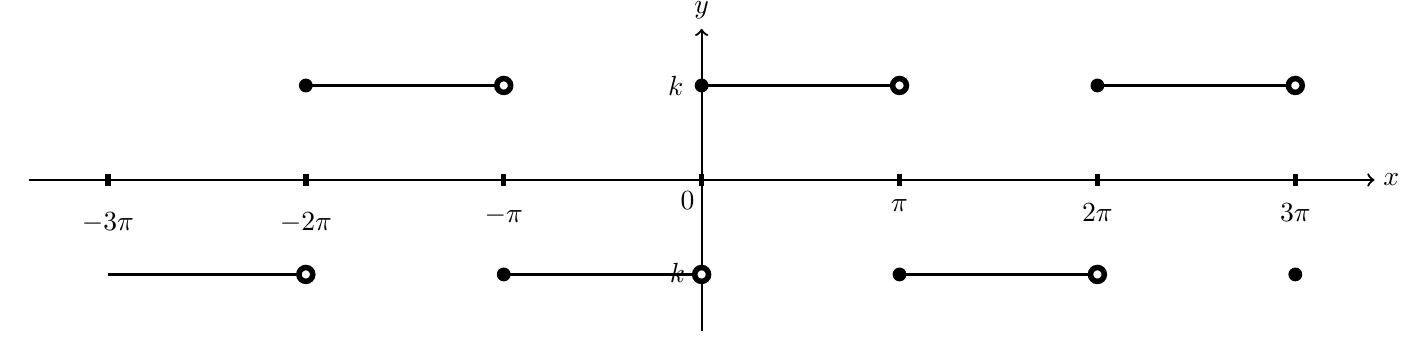
\begin{tikzpicture}[x=0.8cm,y=1cm]
    \pgfmathsetmacro{\p}{pi}
    \def\k{1.2}

    % 座標軸
    \draw[thick,->] ({-3.4*\p},0) -- ({3.4*\p},0) node[right] {$x$};
    \draw[thick,->] (0,{-1.6*\k}) -- (0,{1.6*\k}) node[above] {$y$};

    % x軸の目盛
    \draw ({-3*\p},0.08) -- ({-3*\p},-0.08) node[below] {$-3\pi$};
    \draw ({-2*\p},0.08) -- ({-2*\p},-0.08) node[below] {$-2\pi$};
    \draw ({-\p},0.08) -- ({-\p},-0.08) node[below] {$-\pi$};
    \draw (0,0.08) -- (0,-0.08) node[below left] {$0$};
    \draw ({\p},0.08) -- ({\p},-0.08) node[below] {$\pi$};
    \draw ({2*\p},0.08) -- ({2*\p},-0.08) node[below] {$2\pi$};
    \draw ({3*\p},0.08) -- ({3*\p},-0.08) node[below] {$3\pi$};

    % y軸の目盛
    \draw (0.08,\k) -- (-0.08,\k) node[left] {$k$};
    \draw (0.08,{-\k}) -- (-0.08,{-\k}) node[left] {$-k$};

    % 方形波を3周期分描画
    \foreach \m in {-1,0,1} {
        % 区間 [2m\pi-\pi,\,2m\pi) では -k
        \draw[thick] ({2*\m*\p-\p},{-\k}) -- ({2*\m*\p},{-\k});

        % 区間 [2m\pi,\,2m\pi+\pi) では k
        \draw[thick] ({2*\m*\p},{\k}) -- ({2*\m*\p+\p},{\k});

        % x = 2m\pi での不連続
        \draw[fill=white] ({2*\m*\p},{-\k}) circle (2.5pt);
        \fill ({2*\m*\p},{\k}) circle (2.5pt);

        % x = 2m\pi+\pi での不連続
        \draw[fill=white] ({2*\m*\p+\p},{\k}) circle (2.5pt);
        \fill ({2*\m*\p+\p},{-\k}) circle (2.5pt);
    }
\end{tikzpicture}
\caption{方形波のグラフ}
\end{figure}
\end{document}